
\subsection{Counter examples for the invalid cases}

    For each case where reordering is not safe to do, we also show counter examples of programs where new observable behaviors are introduced.
    This additionally potrays additional proof of the validity of our approach. 

    For all the examples we show here, we only show the ordering relations that are important to observe. 
    Putting all the relations among different events in the example will result in confusion, hence we avoid doing so. 

    \paragraph{Reads to same memory where $e$ is of type $sc$ while $d$ is of either $uo/sc$}
        
        The following example involves two reads to the same memory and a write. 
        
        \begin{figure}[H]
            \centering
            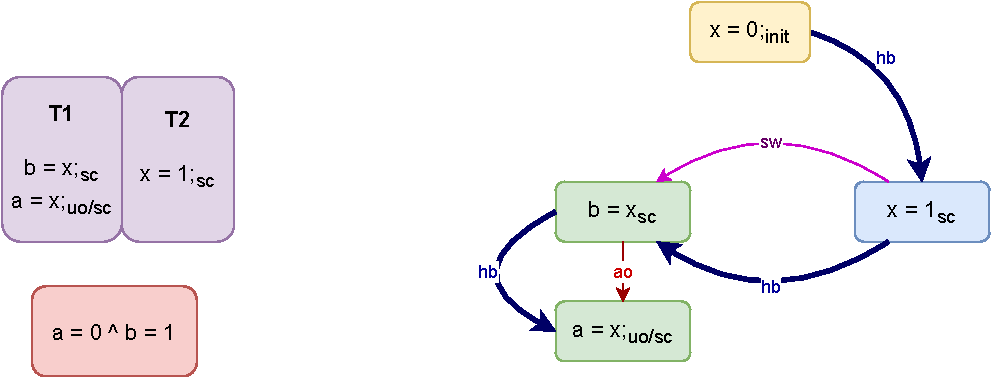
\includegraphics[scale=0.7]{InstructionReordering/Example1(Rsc-Ruo,sc).pdf}
            \caption{Case where a = 0 , b = 1 is invalid due to Coherent Reads}
        \end{figure}

        The figure on the left above shows an example of a candidate where the case of reads in the red box is not possible. 
        The figure on the right shows the Candidate Execution of such a case. 
        Observations:
        \begin{itemize}
            \item We can infer from the Candidate Execution that $\reln{\{x=0_{init}\}}{hb}{\reln{\{x=1_{sc}\}}{hb}{\{a=x_{uo/sc}\}}}$.
            \item By the second axiom of coherent reads, it is not possible for $a$ to read the value of $0$ as $x$ due to the intervening write whiCh changes $x$ to $1$.  
            \item This inference does not rely upon the access mode of the read $a$. 
        \end{itemize}
        
        \begin{figure}[H]
            \centering
            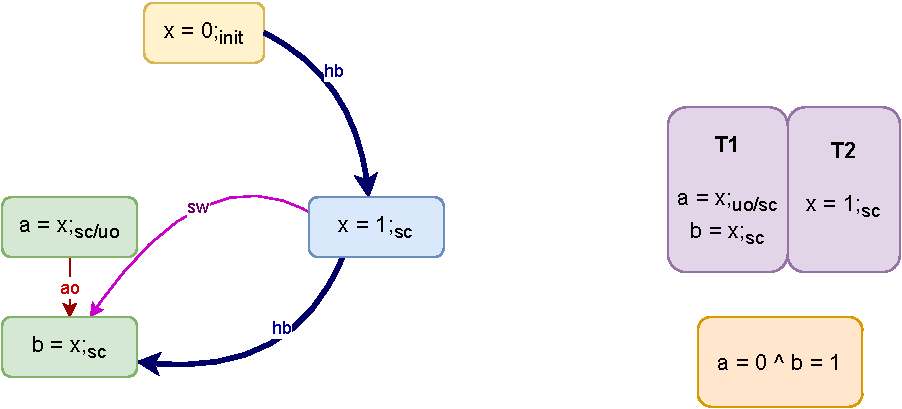
\includegraphics[scale=0.7]{InstructionReordering/Example1R(Rsc-Ruo,sc).pdf}
            \caption{Case where the reads are reordered and a = 0 , b = 1 is valid}
        \end{figure}

        The figure on the left shows the program after reordering the two reads in $T1$, where the case of reads in the orange box is possible. 
        The figure on the right shows the Candidate Execution of such a case. 

        Observations:
        \begin{itemize}
            \item From the Candidate Execution, we can infer $\neg\reln{\{x=0_{init}\}}{hb}{\reln{\{x=1_{sc}\}}{hb}{\{a=x_{uo/sc}\}}}$
            \item We can also infer that $\reln{\{x=0_{init}\}}{hb}{\{a=x_{uo/sc}\}}$    
            \item Since none of the axioms disallow this pattern, $a$ is allowed to read the value of $x$ to be $0$.
            \item Hence, the reordering of the two reads is invalid. 
        \end{itemize}